\documentclass[12pt,a4paper]{article}


% -------------------------------------------------------------------------
% import common LaTeX settings
% -------------------------------------------------------------------------

\usepackage{import}

\subimport{../}{CommonLaTeXSettings}


% -------------------------------------------------------------------------
\begin{document}
% -------------------------------------------------------------------------

\title{
Maintainer's guide to \xmlToLy\ \\[5pt]
}

\author{
Jacques Menu 
}

\date {\normalsize \today\ version}
%\date {}

\maketitle
\thispagestyle{fancy} % right after \maketitle to apply it to the first page too

\abstract {
This document presents the design principles and architecture os \xmlToLy, as well as information needed to maintain it. It is part of the \lib\ documentation, to be found at \url{https://github.com/grame-cncm/libmusicxml/tree/lilypond/doc}. \xmlToBrl\ is mentioned but not described in detail.


In the \lib\ library, the source code specific to \xmlToLy\ can be found at \url{https://github.com/grame-cncm/libmusicxml/tree/lilypond/src/lilypond} and \url{https://github.com/grame-cncm/libmusicxml/tree/lilypond/src/interface}.

All the examples mentioned can be downloaded from \url{https://github.com/grame-cncm/libmusicxml/tree/lilypond/files/samples/musicxml}. They are grouped by subject in subdirectories, such as \mxmlfile{basic/HelloWorld.xml}.
}

% -------------------------------------------------------------------------
% -------------------------------------------------------------------------
\section{Acknowledgements}
% -------------------------------------------------------------------------
% -------------------------------------------------------------------------

Many thanks to Dominique Fober, the designer and maintainer of the \lib\ library!


% -------------------------------------------------------------------------
% -------------------------------------------------------------------------
\section{Overview of \xmlToLy\ }
% -------------------------------------------------------------------------
% -------------------------------------------------------------------------

% -------------------------------------------------------------------------
\subsection{Why \xmlToLy?}
% -------------------------------------------------------------------------

\mxml\ ({\it Music eXtended Markup Language}) is a specification language meant to represent music scores by texts, readable both by humans and computers. It has been designed by the W3C Music Notation Community Group (\url{https://www.w3.org/community/music-notation/}) to help sharing music score files between applications, through export and import mechanisms.

The homepage to \mxml\ is \url{https://www.musicxml.com}.

\mxml\ data contains very detailed information about the music score, and it is quite verbose by nature. This makes creating such data by hand quite difficult, and this is done by applications actually.

% -------------------------------------------------------------------------
\subsection{What \xmlToLy\ does}
% -------------------------------------------------------------------------


% -------------------------------------------------------------------------
% -------------------------------------------------------------------------
\section{Prerequisites}
% -------------------------------------------------------------------------
% -------------------------------------------------------------------------

In order to maintain \xmlToLy, one needs to do the following:
\begin{itemize}
\item obtain a working knowledge of C++ programming. The code base of \xmlToLy\ uses classes, simple and multiple inheritance, and templates;

\item study \mxml, starting maybe from \docpdf{introductionToMusicXML}{IntroductionToMusicXML.tex}. A deep knowledge of that matter comes with experience;

\item study the architecture of \lib, which can be seen at \docpdf{libmusicxmlArchitecture}{libmusicxmlArchitecture.pdf}, and is presented in figure \ref{libmusicxmlArchitecture}.
It shows the place of \xmlToLy\ in the whole.

\item
\end{itemize}

\begin{figure}
\caption{\lib\ architecture}\mylabel{libmusicxmlArchitecture}
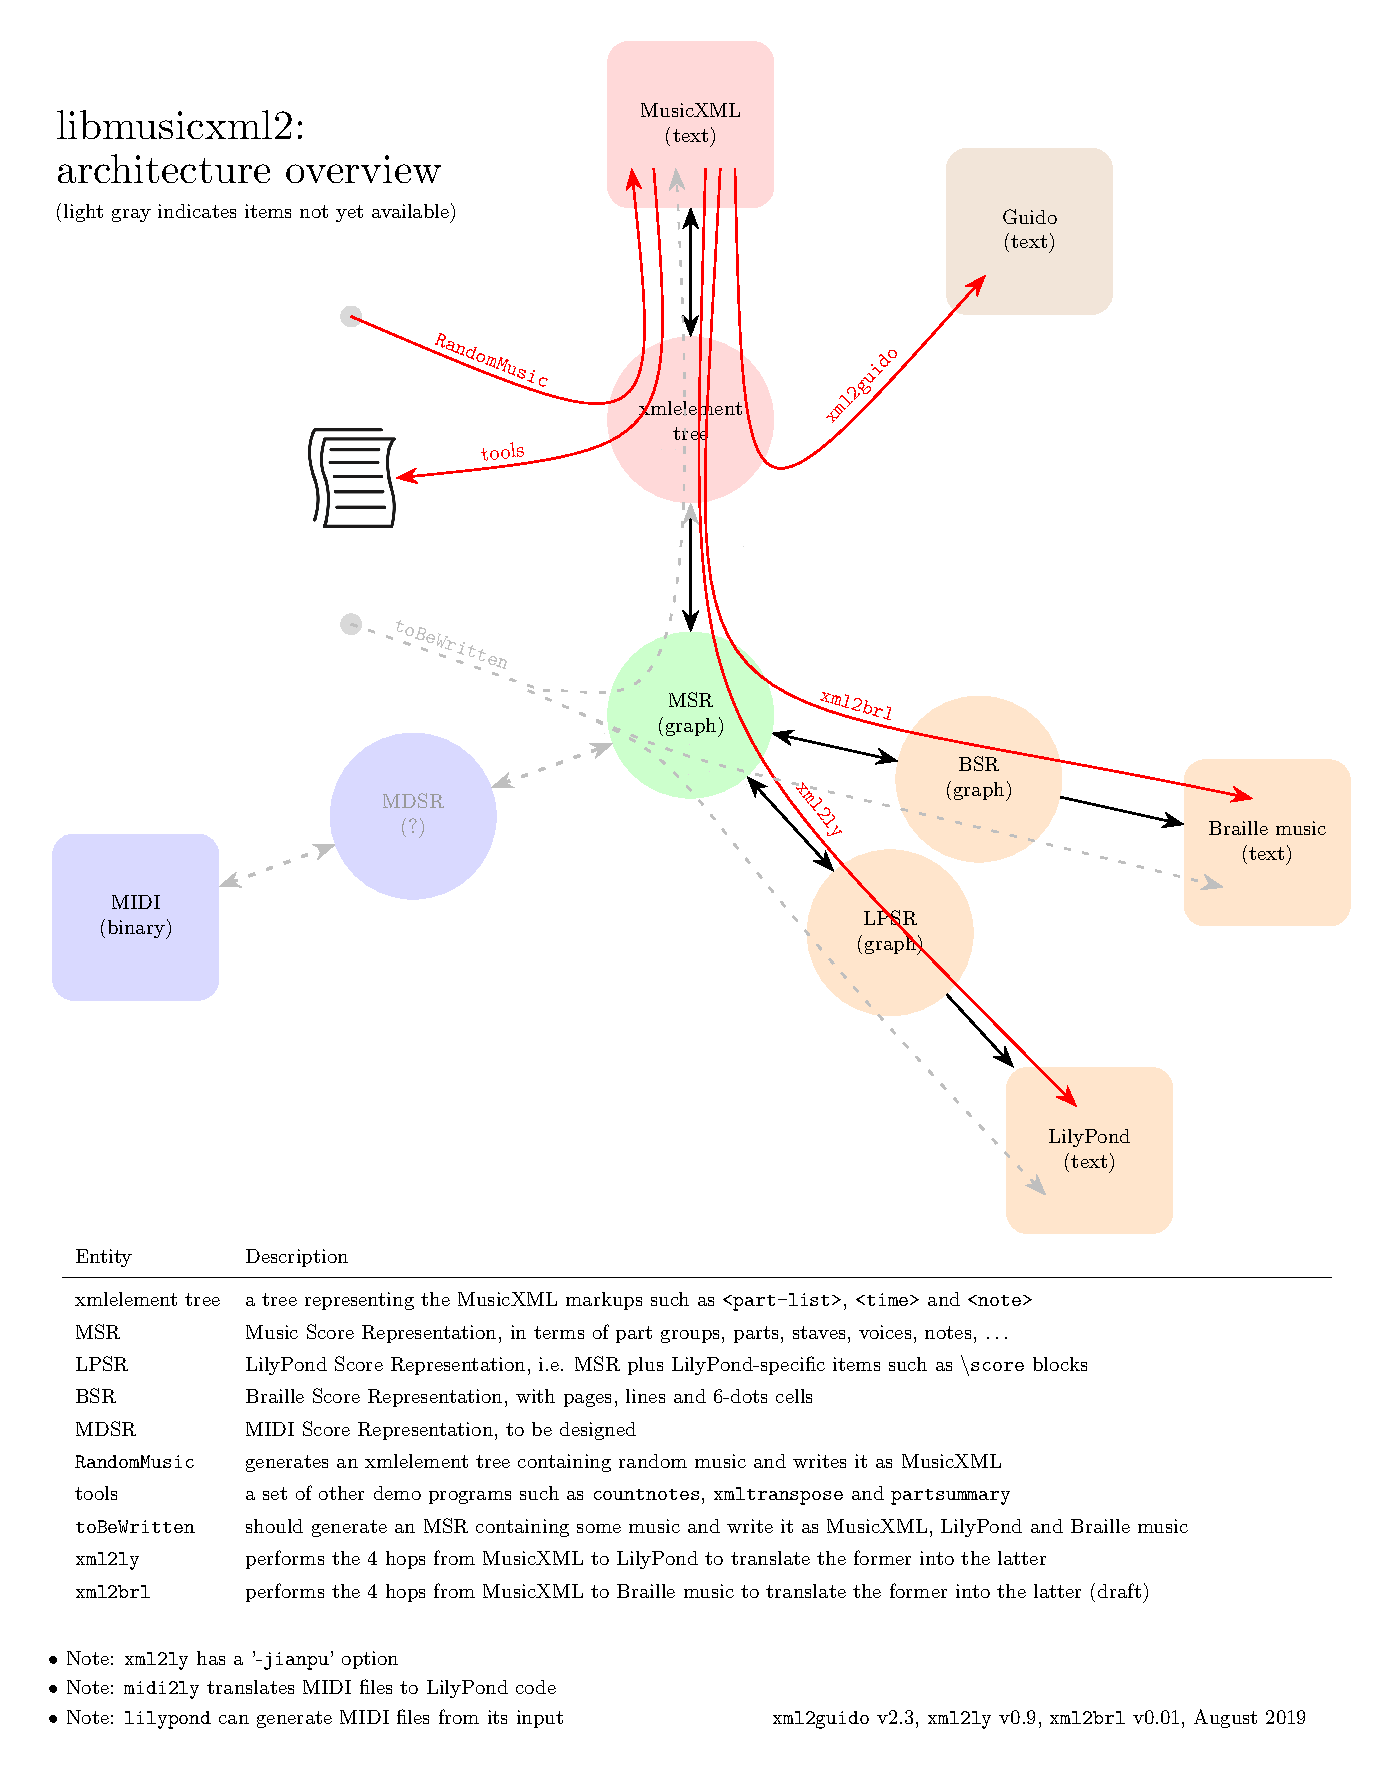
\includegraphics[scale=0.8]{../libmusicxmlArchitecture/libmusicxmlArchitecture.pdf}
\end{figure}


% -------------------------------------------------------------------------
% -------------------------------------------------------------------------
\section{Programming style and conventions}
% -------------------------------------------------------------------------
% -------------------------------------------------------------------------

% -------------------------------------------------------------------------
\subsection{Source code presentation}
% -------------------------------------------------------------------------

The following text-editing conventions are used:
\begin{itemize}
\item tabs are not used before the first non-space character in a line, two spaces are used instead;

\item the code is not tightly packed: declarations in classes have the members' names aligned vertically, with many spaces before them if needed, and empty lines are used to separate successive activities in methods.
\end{itemize}

% -------------------------------------------------------------------------
\subsection{File names}
% -------------------------------------------------------------------------

The name '{\tt lilypond}' was chosen by Dominique long before work started on \\xmlTobrl.

There's a single '{\tt lilypond}' folder to contain MSR, LPSR, BSR, \xmlToLy\ and \xmlToBrl, even though BSR and braille music are a distinct branch. This has been preferred by Dominique as the manager of \lib.

Most file names start with an identification of the context they belong to, such as '{\tt oah}', '{\tt mxmlTree}', '{\tt msr}', '{\tt lpsr}', '{\tt lilypond}', '{\tt bsr}', '{\tt braille}', '{\tt xml2ly}' and '{\tt xml2brl}'.

The '{\tt *Oah.*}' files handle the options and help for the corresponding context, such as '{\tt xml2lyOah.h/.cpp}'.

The '{\tt traceOah.h/.cpp}', '{\tt musicXMLOah.h/.cpp}', '{\tt extra}' and '{\tt general}' context are about the corresponding help groups.

There are a couple of 'globlal' files not related to any particular context: '{\tt utilities.h/.cpp}', '{\tt messagesHandling.h/.cpp}' and '{\tt version.h/.cpp}'.


% -------------------------------------------------------------------------
\subsection{Defensive programming}
% -------------------------------------------------------------------------

The code base of \xmlToLy\ is {\it defensive programming} oriented, which means that:
\begin{itemize}
\item identifiers are explicit and long if needed -- only very local ones are short, such as iteration loops indexes;

\item the code is organized in sections, with an initial comment documenting what the code does;

\item '{\tt msrAssert()}' is used to do sanity checks, such as detect a null pointer prior to using it;
\end{itemize}

The \mxml\ data is not systematically checked for correctness. Checks are done, however, to ensure it won't crash due to missing values.


% -------------------------------------------------------------------------
% -------------------------------------------------------------------------
\section{The two-phase visitors pattern}
% -------------------------------------------------------------------------
% -------------------------------------------------------------------------

% -------------------------------------------------------------------------
\subsection{Basic mechanism}
% -------------------------------------------------------------------------

% -------------------------------------------------------------------------
\subsection{An example}
% -------------------------------------------------------------------------


% -------------------------------------------------------------------------
% -------------------------------------------------------------------------
\section{Passes organization}
% -------------------------------------------------------------------------
% -------------------------------------------------------------------------


% -------------------------------------------------------------------------
% -------------------------------------------------------------------------
\section{Translating \mxml\ data to an \mxmlt}
% -------------------------------------------------------------------------
% -------------------------------------------------------------------------


% -------------------------------------------------------------------------
% -------------------------------------------------------------------------
\section{Translating an \mxmlt\ to an MSR}
% -------------------------------------------------------------------------
% -------------------------------------------------------------------------


% -------------------------------------------------------------------------
% -------------------------------------------------------------------------
\section{Translating an an MSR to a LPSR}
% -------------------------------------------------------------------------
% -------------------------------------------------------------------------


% -------------------------------------------------------------------------
% -------------------------------------------------------------------------
\section{Translating an an LPSR to a LilyPond code}
% -------------------------------------------------------------------------
% -------------------------------------------------------------------------



% -------------------------------------------------------------------------
% -------------------------------------------------------------------------
% postamble
% -------------------------------------------------------------------------
% -------------------------------------------------------------------------

\pagebreak

\lstlistoflistings

\listoffigures

\tableofcontents


% -------------------------------------------------------------------------
\end{document}
% -------------------------------------------------------------------------
